\subsection{Model Animation} \label{sec:theory_theory_models_animation}
Model animations make use of a \textit{model armature} (also called \textit{skeleton}) which can be seen in \autoref{fig:armature}.
The armature is a set of bones that have different relations to each other and the mesh.
The bones create a tree structure with the root being the torso bone.
Most other bones are children of the torso bone or children of children of the torso bone.
This relation allows the bones to inherit transformations from their parents.
For example, if a leg bone moves the foot bone will follow.

It is worth noting that bone structure does not have to resemble the human bone structure.
For example in \autoref{fig:armature_foot} we can see a set of bones that are outside of the body.
These bones are not used to deform the mesh but to interact with other bones.
Among other things, these guarantee that the knee does not bend in the wrong direction.


\begin{figure}[h]
    \centering
    \begin{subfigure}{0.45\textwidth}
        \centering
        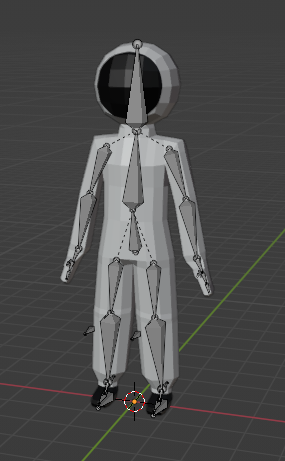
\includegraphics[width=0.8\textwidth]{chapters/theoretical_foundations/sections/models/resources/Armature.png}
        \caption{Armature.}
        \label{fig:armature}
    \end{subfigure}
    \hfill
    \begin{subfigure}{0.45\textwidth}
        \centering
        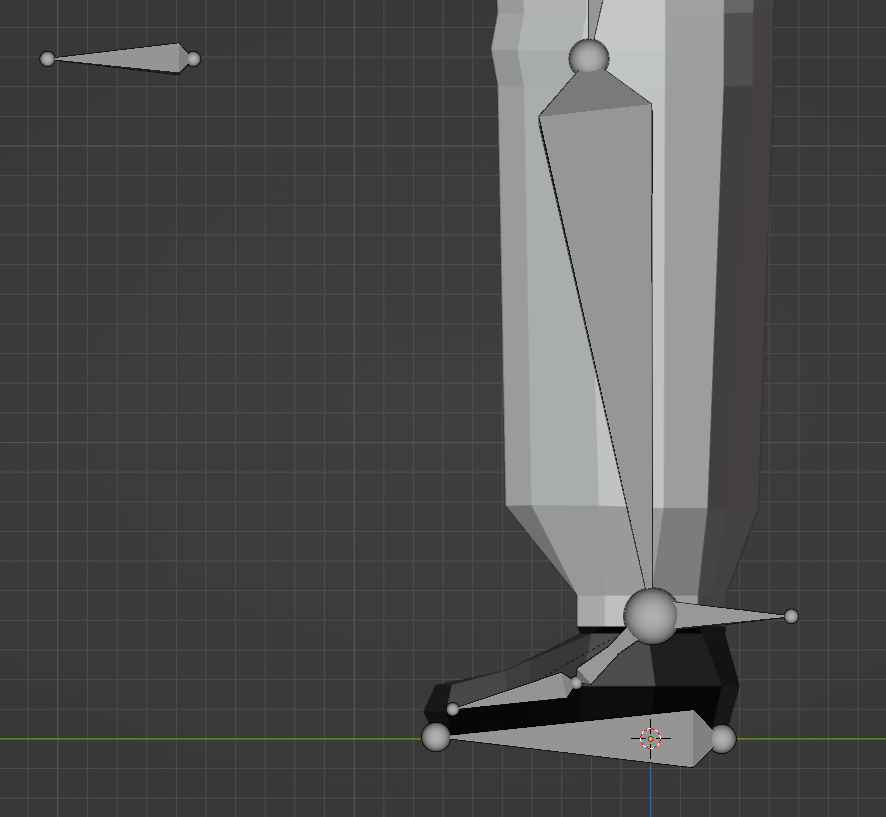
\includegraphics[width=0.8\textwidth]{chapters/theoretical_foundations/sections/models/resources/ArmatureFoot.png}
        \caption{Abnormal bones.}
        \label{fig:armature_foot}
    \end{subfigure}

    \caption{Armature.}
\end{figure}

The bones need to be connected to the mesh.
Each vertex is assigned a set of bones that influence it with different weights.
When bones move the vertices move with them according to how much they move and how much a certain bone influences a certain vertex.
Assigning weights to vertices in Blender is shown in \autoref{fig:vertex_weights}.
As can be seen in the figure, it is done by selecting a bone and then painting the vertices with a certain weight.

\begin{figure}[h]
    \centering
    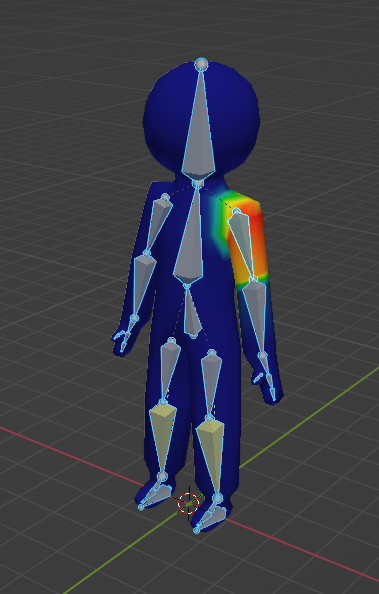
\includegraphics[width=0.45\textwidth]{chapters/theoretical_foundations/sections/models/resources/WeightPaint.png}
    \caption{Vertex weights.}
    \label{fig:vertex_weights}
\end{figure}

To define an animation a set of \textit{keyframes} is used.
The process of creating the keyframes can be seen in \autoref{fig:keyframes}.
A keyframe is a set of transformations for each bone at a certain time.
Once the keyframes are defined the animation is interpolated between them to produce a smooth animation.
In the game, there are two animations: walking and running, both of which are looped to create a continuous animation when the player or an NPC moves.

\begin{figure}[h]
    \centering
    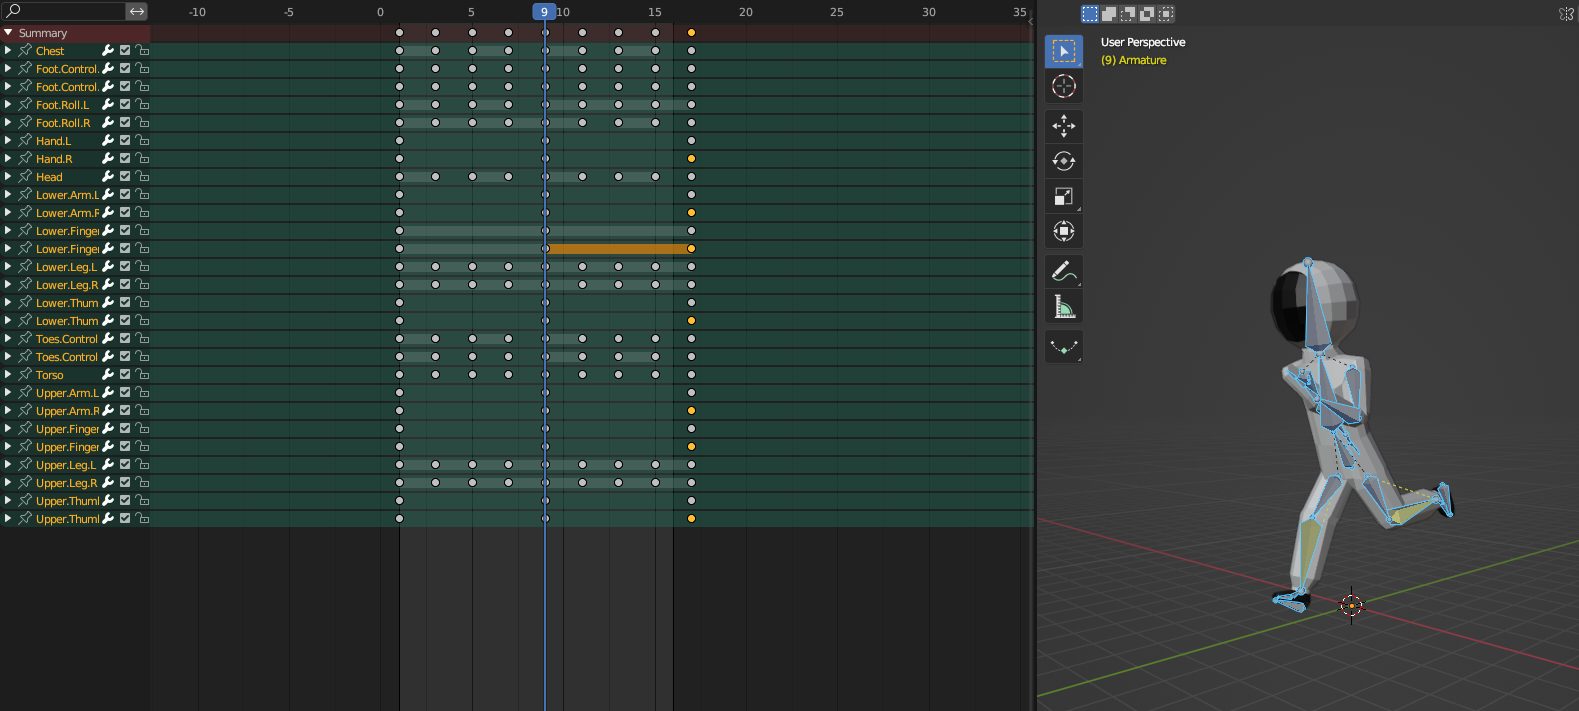
\includegraphics[width=1\textwidth]{chapters/theoretical_foundations/sections/models/resources/DopeSheet.png}
    \caption{Keyframes.}
    \label{fig:keyframes}
\end{figure}


The whole process of rendering an animation is as follows:
\begin{enumerate}
    \item The model along with the armature and keyframes are loaded into the game.
    \item The timer is started.
    \item The bone transformations for the current frame are calculated based on the keyframes and the timer, by interpolating between the keyframes.
    \item The bone transformations are passed into the shader.
    \item For each vertex the shader iterates over the bones that influence it and calculates the final position of the vertex based on the bone transformations and their weights.
    \item The animation is rendered.
\end{enumerate}